\documentclass[a4paper]{article}
\setlength{\parindent}{0.0pt}
\usepackage{amsfonts}
\usepackage{listings}

\usepackage{graphicx}
\usepackage[american]{babel}
\usepackage[T1]{fontenc}
\usepackage[utf8x]{inputenc}

\newcommand{\TITLE}{SWAG - Assignment 3}
\newcommand{\AUTHOR}{
  Philipp Raich, \emph{0404014}\\
  Frieder Ulm, \emph{0527031}\\
	Matthias Steinböck, \emph{0527943}\\
	Hubert Hirsch, \emph{0625008}\\
	Eugen Dahm, \emph{0625325} 
}
\newcommand{\GROUP}{swa043}
\newcommand{\SUBJECT}{Software Architecture}
\newcommand{\KEYWORDS}{Software Architecture, Patterns, }
\newcommand{\MAIL}{
\href{mailto:e0404014@student.tuwien.ac.at}
{e0404014@student.tuwien.ac.at}\\
\href{mailto:e0527031@student.tuwien.ac.at}
{e0527031@student.tuwien.ac.at}\\
\href{mailto:e0527943@student.tuwien.ac.at}
{e0527943@student.tuwien.ac.at}\\
\href{mailto:e0625008@student.tuwien.ac.at}
{e0625008@student.tuwien.ac.at}\\
\href{mailto:e0625325@student.tuwien.ac.at}
{e0625325@student.tuwien.ac.at}
}
\newcommand{\HRule}{\rule{\linewidth}{0.25mm}}

\usepackage{hyperref}

\hypersetup
{
  pdftitle  = {\TITLE},
  pdfsubject  = {\SUBJECT},
  pdfauthor   = {\AUTHOR},
  pdfkeywords = {\KEYWORDS},
  colorlinks  = false,
  linkcolor   = black,
  anchorcolor = black,
  citecolor   = black,
  urlcolor  = black
}

\begin{document}

\begin{titlepage}

\begin{center}

% Upper part of the page
%\includegraphics[width=0.15\textwidth]{./logo}\\[1cm]    
\begin{figure}[ht!]
  \begin{center}
  
\includegraphics[width=1\textwidth]{fig/vitalab-header.png}
  \label{fig:component_diagram}
  \end{center}
\end{figure}

\textsc{\LARGE TU Vienna}\\[1.5cm]

\textsc{\Large Software Architecture}\\[0.5cm]


% Title
\HRule \\[0.4cm]
{ \huge \bfseries \TITLE}\\[0.15cm]

\HRule \\[1.5cm]

% Author and supervisor
\emph{Authors:}\\
\large{\AUTHOR\\}
\vfill
\normalsize\emph{Group:}
\large\textbf{\GROUP}\\

\vfill

% Bottom of the page
{\normalsize \today}

\end{center}

\end{titlepage}

\section{Use Cases}

The following Use Cases where identified and implemented

\begin{tabular}[t]{|l|l|p{7cm}|}
\hline
\textbf{Use Case}	&	\multicolumn{2}{|l|}{\textbf{Create User Account}}\\
\hline
Goal in Context	&	\multicolumn{2}{|l|}{User can create a account}\\
\hline
Additional Notes	&	\multicolumn{2}{|p{10cm}|}{Starting base is initialized, user gets an e-mail with his generated password}\\
\hline
\end{tabular}\\

\begin{tabular}[t]{|l|l|l|}
\hline
\textbf{Use Case}	&	\multicolumn{2}{|l|}{\textbf{Delete User Account}}\\
\hline
Goal in Context	&	\multicolumn{2}{|l|}{User can delete his account}\\
\hline
Additional Notes	&	\multicolumn{2}{|l|}{Bases are abandoned and can be taken by other players}\\
\hline
\end{tabular}\\

\begin{tabular}[t]{|l|l|p{7cm}|}
\hline
\textbf{Use Case}	&	\multicolumn{2}{|p{7cm}|}{\textbf{Login/Logout}}\\
\hline
Goal in Context	&	\multicolumn{2}{|p{7cm}|}{User can Login/Logout on/off his account}\\
\hline
Additional Notes	&	\multicolumn{2}{|p{10cm}|}{Game State must be saved correctly until next Login, while the game continues and already taken actions continue}\\
\hline
\end{tabular}\\

\begin{tabular}[t]{|l|l|l|}
\hline
\textbf{Use Case}	&	\multicolumn{2}{|l|}{\textbf{Send Ingame Message}}\\
\hline
Goal in Context	&	\multicolumn{2}{|l|}{User can send ingame messages to other users}\\
\hline
\end{tabular}\\

\begin{tabular}[t]{|l|l|l|}
\hline
\textbf{Use Case}	&	\multicolumn{2}{|l|}{\textbf{Receive Ingame Message}}\\
\hline
Goal in Context	&	\multicolumn{2}{|l|}{User can receive ingame messages from other users}\\
\hline
\end{tabular}\\

\begin{tabular}[t]{|l|l|l|}
\hline
\textbf{Use Case}	&	\multicolumn{2}{|l|}{\textbf{Build Base}}\\
\hline
Goal in Context	&	\multicolumn{2}{|l|}{User can build base on a map}\\
\hline
\end{tabular}\\

\begin{tabular}[t]{|l|l|l|}
\hline
\textbf{Use Case}	&	\multicolumn{2}{|l|}{\textbf{Build Building}}\\
\hline
Goal in Context	&	\multicolumn{2}{|l|}{User can build building on a base}\\
\hline
\end{tabular}\\

\begin{tabular}[t]{|l|l|l|}
\hline
\textbf{Use Case}	&	\multicolumn{2}{|l|}{\textbf{Upgrade Building}}\\
\hline
Goal in Context	&	\multicolumn{2}{|l|}{User can upgrade his existing buildings}\\
\hline
\end{tabular}\\

\begin{tabular}[t]{|l|l|l|}
\hline
\textbf{Use Case}	&	\multicolumn{2}{|l|}{\textbf{Navigate Maps}}\\
\hline
Goal in Context	&	\multicolumn{2}{|l|}{User can navigate through existing maps}\\
\hline
\end{tabular}\\

\begin{tabular}[t]{|l|l|l|}
\hline
\textbf{Use Case}	&	\multicolumn{2}{|l|}{\textbf{Build Troops}}\\
\hline
Goal in Context	&	\multicolumn{2}{|l|}{User can build troops}\\
\hline
\end{tabular}\\

\begin{tabular}[t]{|l|l|l|}
\hline
\textbf{Use Case}	&	\multicolumn{2}{|l|}{\textbf{Form Squad}}\\
\hline
Goal in Context	&	\multicolumn{2}{|l|}{User can form squads with built troops}\\
\hline
\end{tabular}\\

\begin{tabular}[t]{|l|l|l|}
\hline
\textbf{Use Case}	&	\multicolumn{2}{|l|}{\textbf{Move Squads}}\\
\hline
Goal in Context	&	\multicolumn{2}{|l|}{User can move his sqauds to other squares}\\
\hline
Additional Notes	&	\multicolumn{2}{|p{10cm}|}{Squares occupied by foreign squads will be attacked by moving there, the "stronger" squads win, defeated troops disappear, if only foreign buildings remain on the square, they are attacked and will dissapear, remaning resources are assigned to the attacker}\\
\hline
\end{tabular}\\

\clearpage

\section{Issues and Decisions}

\begin{tabular}[t]{|l|p{10cm}|}
\hline
\textbf{Issue}	&	The Application must be able to scale according to a unknown player count\\
\hline
Decision & Server load is minimized through gui-rendering executed client-side (html-prefetch \& JavaScript)\\
\hline
Status	& Implemented\\
\hline
Constraints	&	None\\
\hline
Related Principles	&	Thick Client\\
\hline
Related Artifacts	&	GUI\\
\hline
\end{tabular}\\

\begin{tabular}[t]{|l|p{10cm}|}
\hline
\textbf{Issue}	&	Reliable and fast communication between GUI and Business Logic to minimize overhead and loading times\\
\hline
Decision	&	JSON-Format mesaging between GUI (Client) and Business Logic (Server)\\
\hline
Status	& Implemented\\
\hline
Constraints	&	None\\
\hline
Related Principles	&	Thick Client\\
\hline
Related Artifacts	&	All GUI-related Components\\
\hline
\end{tabular}\\

\begin{tabular}[t]{|l|p{10cm}|}
\hline
\textbf{Issue}	&	The application must be extensible\\
\hline
Decision & New modules and Services can easily be implemented in the exisiting structure\\
\hline
Status	& Implemented\\
\hline
Constraints	&	None\\
\hline
Related Principles	&	Extensibility\\
\hline
Related Artifacts	&	All\\
\hline
\end{tabular}\\

\subsection{Implementation Details}

Application Server: \textbf{Glassfish 3.1}\\
Database: \textbf{PostgreSQL 8.4}\\
Client-Side (Rendering): \textbf{AJAX}\\

The following JavaScript Libraries were used:
\begin{itemize}
\item jquery
\item requirejs
\item jquery.cookie
\item jquery.bind
\item jquery.ui
\item md5
\end{itemize}


\clearpage

\section{Component Diagram}

\begin{figure}[ht!]
  \begin{center}
  \hspace*{-90pt}
  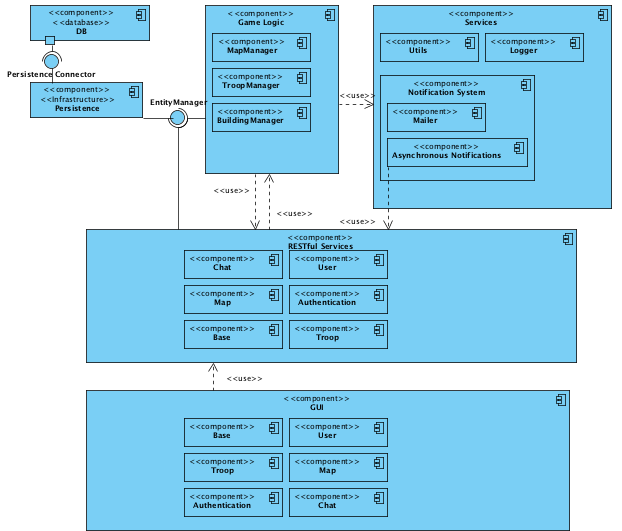
\includegraphics[scale=0.60]{fig/components.png}
  \label{fig:component_diagram}
  \caption{SWAG Component Diagram}
  \end{center}
\end{figure}

\hspace*{0pt}

\clearpage

%\section{Deployment Diagram}
%\clearpage

\section{Database Model}

\begin{figure}[ht!]
  \begin{center}
  \hspace*{-90pt}
  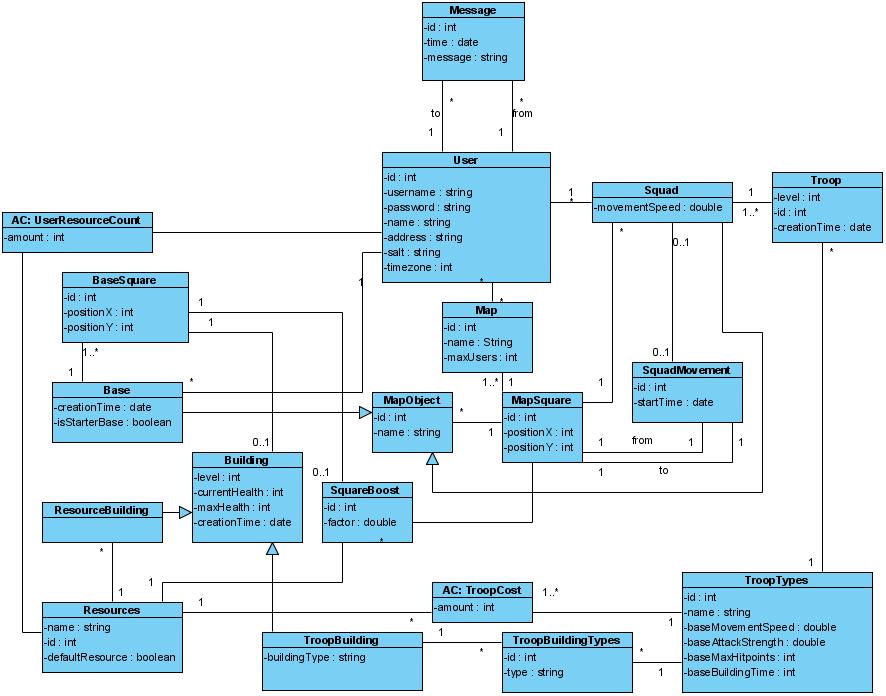
\includegraphics[scale=0.55]{fig/database_model.png}
  \label{fig:database_model}
	\caption{SWAG Database Model}
  \end{center}
\end{figure}

\hspace{0pt}

%\bibliographystyle{IEEEbib}
%\bibliography{bibtex}

\end{document}
